\documentclass[a4paper]{scrreprt}
\usepackage{etex}
\usepackage[utf8]{inputenc}
%\usepackage[T1]{fontenc}
\usepackage{lmodern}
\usepackage{hyphsubst}
\usepackage[english]{babel}
\usepackage{textcomp}
\usepackage{enumerate}
\usepackage{microtype}
\usepackage{listings}
\usepackage{graphicx}
\usepackage{subcaption}
\usepackage{titling}
\usepackage{amsmath}
\usepackage{float}
\lstset{language=[LaTeX]TeX}

\usepackage{wallpaper}

\renewcommand{\quote}[1]{``#1''}

\begin{document}
\URCornerWallPaper{0.25}{TUHH.png}
\title{Report on Exam Task\\Simulation and Modelling of Communication Networks}
\author{Nicolás Chopitea Kober, Sebastian Lindner}
\date{Summer Term 2016}
\maketitle	

\tableofcontents
\newpage

\chapter{Overview}
\section{Description}
	We were tasked by a university to analyze the usefulness, practicability and limitations of a remote university building's direct radio link to the main university campus. 
	
	In this chapter we will attempt to fully capture the scenario at hand, abstract it into a model and extract the requirements that have to be fulfilled in order to have an applicable solution to connecting the remote building with the main campus via radio.
\section{Requirement Analysis}
	\subsection{Network Description}
		The aim is to connect a remote building's network to the main university campus network. The fast cabled connection is endangered due to a construction site in close proximity to the building. That is why a direct radio link could be employed to maintain connectivity throughout the construction process.
		
		The following network usage cases could be identified:
		
		\begin{description}
		\item[CCTV] A CCTV camera is connected to the remote building's router. \\ It is continuously transmitting a livestream of its video.
		
		\item[Wireless] A wireless access point operating on the \emph{802.11g} standard is connected to the remote building's router. \\Connected to this access point are users engaged in the following three activities.
		\begin{description}
			\item[FTP Upload] A single file upload can be observed that is ongoing throughout the simulation of the network.
			\item[Video Livestream] A remotely located professor is livestreaming his or her lecture to a video conference laptop. \\This connection is bidirectional so that participating students can ask questions.
			\item[Web Browsing] A variable number of students browsing the web is connected to the access point at any time.
		\end{description}
		\end{description}
		
		This describes the network inside the remote building that we are trying to connect. The main campus' network can currently be simplified to three connections:
		
		\begin{description}
			\item[Remote Professor] A fast connection to the remotely located professor's laptop is established via the Deutsches Forschungsnetz. \\It will communicate with the video conference laptop inside the remote building.
			\item[Porter's Office] A CCTV monitoring station sits in the porter's office. \\The livestream of the remote building's CCTV camera will travel here.
			\item[Internet] A VDSL connection to the Internet is present. \\Both web browsing and FTP upload traffic will have this destination.
		\end{description}
		
		A graphical representation of the scenario is as follows and includes technical details such as channel delay and bandwidth:
		
		\begin{figure}[H]
		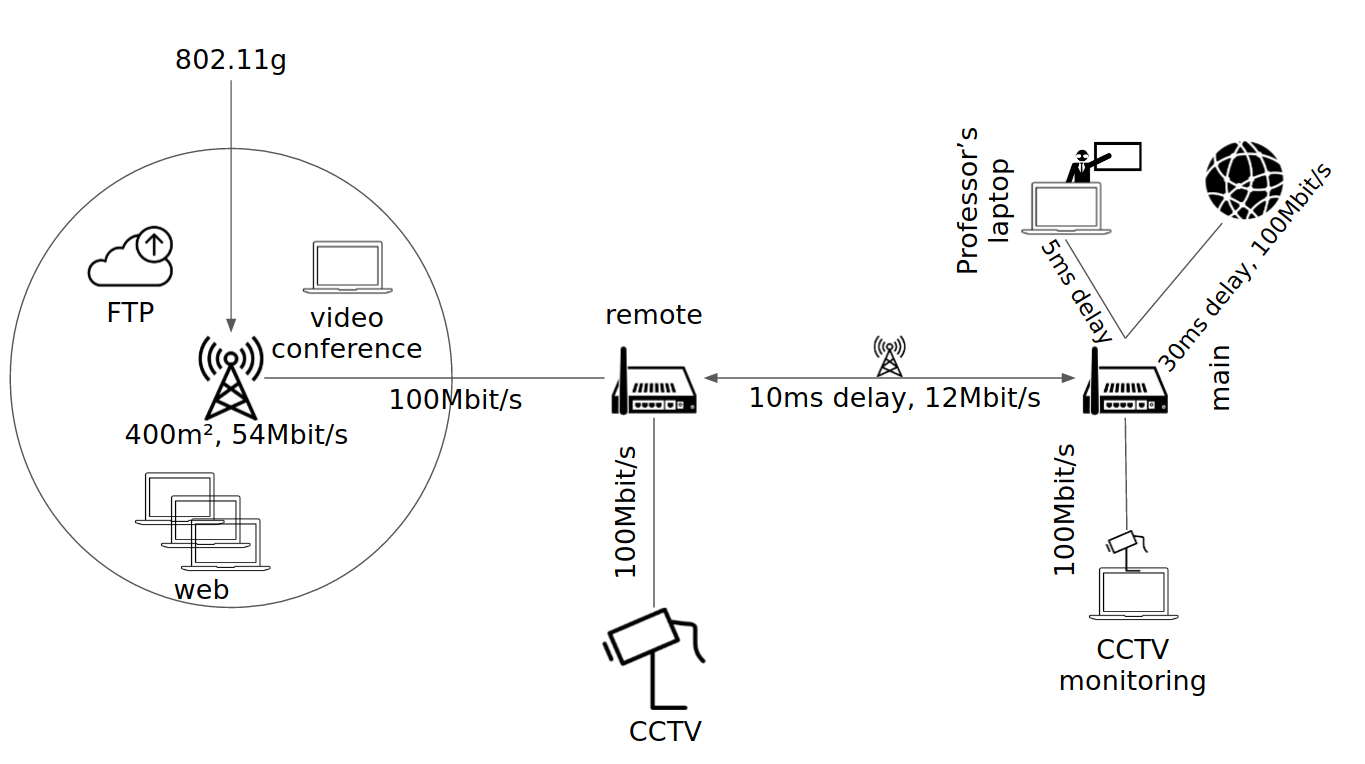
\includegraphics[width=\textwidth]{./simmodel.png}
		\caption{A model of the scenario depicted}
		\end{figure}
	\subsection{Statistical Web Browsing Model}
		The student's web browsing behavior is difficult to capture. We are going to model it by assuming a student issues an HTTP request, receives a response and then spends some time reading the response that is exponentially distributed. Missing at this point is the size of the response that follows a request. To model this we have analyzed a trace file containing 1000 response size values.
		
		We have chosen the \emph{chi squared goodness of fit test} to evaluate how well a distribution fits the observed data. As a first step we investigated the density of values within request size intervals. These intervals initially were of equal size and the observed values were associated to an interval that they lied in. To remove intervals with no values associated to them, these were merged with neighboring intervals. In this way we obtained 160 intervals of which most have observed values associated to them. This is a graphical representation of what we found:
		\begin{figure}[H]
		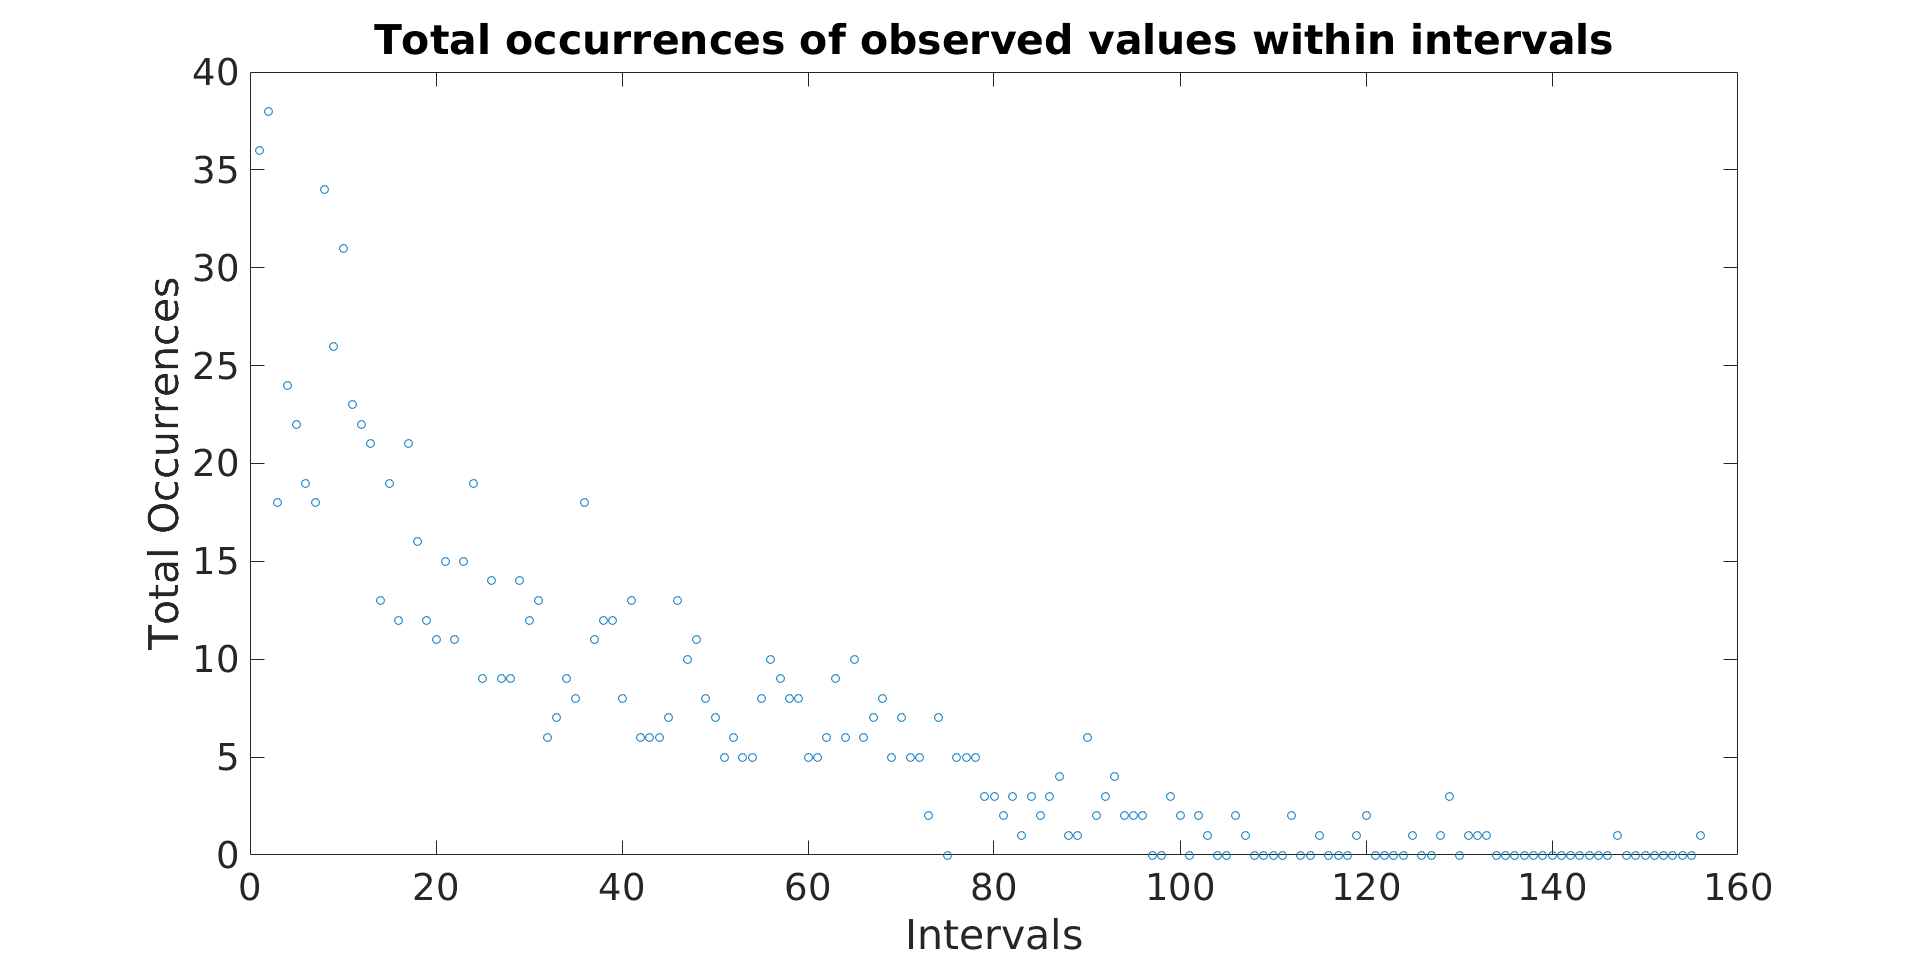
\includegraphics[width=\textwidth]{../tracefile_analysis/exp.png}
		\caption{Request size value density in intervals}
		\end{figure}
		
		We have the highest density of observed values in regions of low response sizes, and the number of observations decreases exponentially for increasing response sizes. This looks closely related to values coming from a \emph{negative exponential distribution}, which is why we decided to apply the test against this distribution.
		
		The test states that the observed values follow an Exponential distribution with mean $\lambda=580390\,\text{Byte}$ at a significance level of $99.95\%$.
		
	\subsection{Open Questions}\label{sec:openquestions}
		We have now modeled the scenario at hand. What remains unclear is
		
		\begin{enumerate}
			\item What number of students can the network handle?
			\item What are the bottlenecks of the network?
			\item How is the lecture livestream's error rate correlated to the number of students?
			\item What impact does the CCTV livestream have on the network?
			\item What impact does the FTP upload have on the network?
		\end{enumerate}
		
		In the next chapter we will try and answer these questions.

\chapter{Simulation}
	We are going to answer the open questions from section \ref{sec:openquestions} through simulation. For this we have modeled the scenario using the \emph{omnet++} simulator.
	
	\section{Configuration}
		We have set up the simulations in the following ways.
		\begin{description}
			\item[Simulation Time] Deciding upon a reasonable simulation time is essential. There are several different protocols in use here. The \emph{802.11g WLAN standard} has, for example, a certain time that it takes until handshakes are complete and regular transmission can start.			
			
			That is why we have simulated the scenario for an extensive period of $5000\text{s}$ to see how throughput fluctuates in which time frames. Figure \ref{fig:5000s} shows the throughput of the remotely located Professor's laptop that livestreams his lecture to the remote building's conference laptop. We chose this use case as it represents the most time critical of all:
			
			\begin{figure}[H]
				\center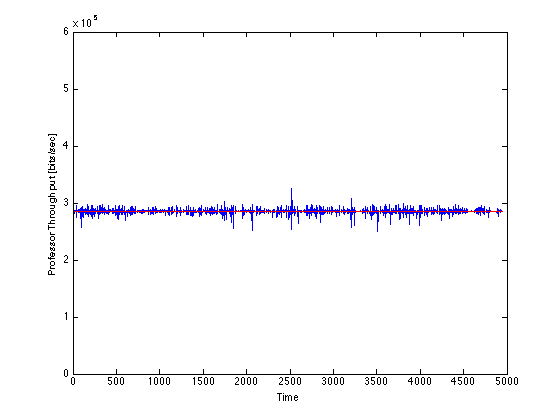
\includegraphics[width=\textwidth]{../Get_Simulation_Parameters/long_simulation_5000sec.png}
				\caption{Throughput over $5000\text{s}$}
				\label{fig:5000s}
			\end{figure}
			
			Our approach to this problem looks like this:
			
			We want to find a simulation time $t$ so that if we went through the throughput depicted in figure \ref{fig:5000s} and sliced it into time intervals of length $t$ - in a sliding window-like manner, and then averaged the throughput values inside the sliding windows, we want these means to be relatively close to each other. This would mean that our $t$ is large enough so that it does not matter much which sliding window we took, the result would be more or less the same. This is equivalent to looking at the variance of these mean values. We applied this procedure on the data from the $5000\text{s}$ run for all $t\in\{250\text{s},\, 350\text{s},\, 500\text{s},\, 750\text{s},\, 1000\text{s}\}$. The result can be seen in figure \ref{fig:relativevariance}.
			
			\begin{figure}[H]
				\center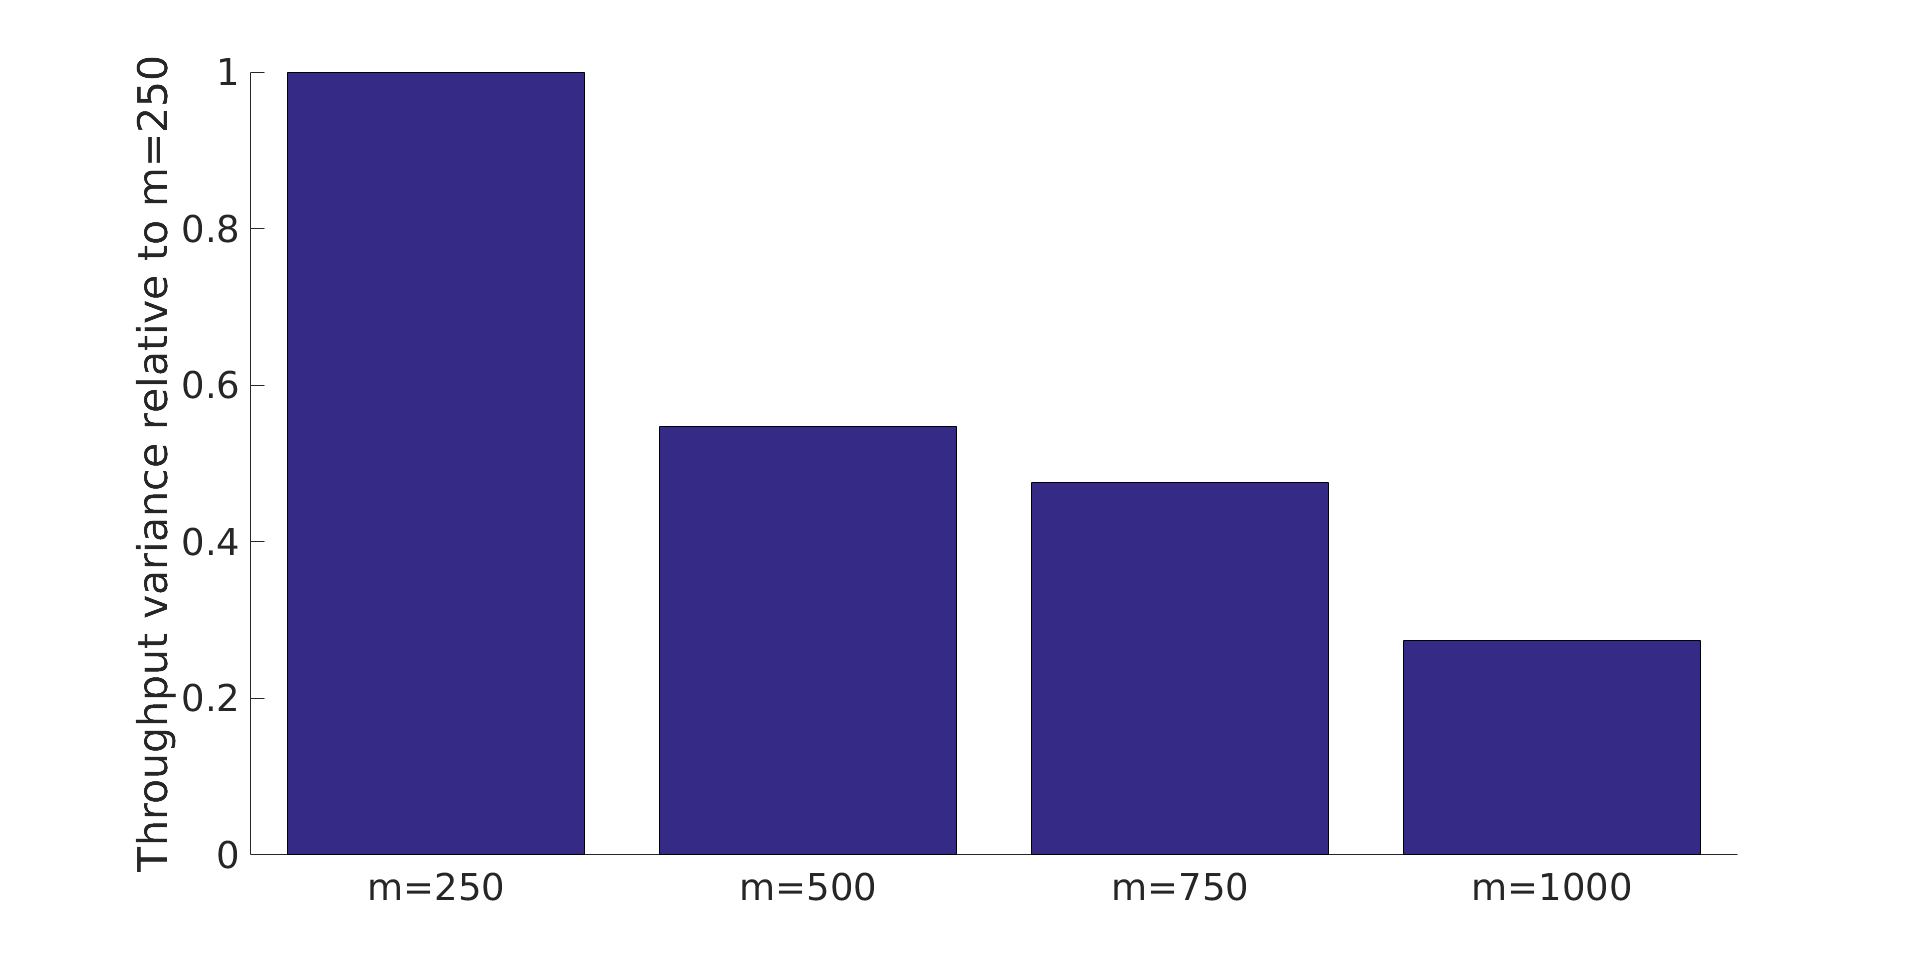
\includegraphics[width=\textwidth]{../Get_Simulation_Parameters/relative_variance.png}
				\caption{Relative variance of sliding window throughput means, where windows were of length $t$, on $5000\text{s}$ data}
				\label{fig:relativevariance}
			\end{figure}
			
			One can observe that doubling $t$ from $t=250\text{s}$ to $t=500\text{s}$ roughly halves the variance. Increasing it further greatly increases the time required to run these simulations while gaining relatively little.
			
			This led us to the decision of setting the simulation time $t=500\text{s}$.
			
			\item[Number of Repetitions] As simulations rely on random events and those build upon pseudo-random numbers that we generate, it is important to run each and every simulation several times with new seeds for the random number generators in order to cover a meaningful number of possibilities with the goal of approximating real world behavior. 
			
			Each run's performance is recorded and denoted as a \emph{sample}. Following the \emph{Central Limit Theorem} we can assume a sample mean to stem from a \emph{Normal distribution}. 
			
			A sample mean estimate
			\[\mu_m=\frac{1}{m}\sum^m_{j=1}y_j\]
			where $m=\text{number of samples}$
			\\and $y_i=\text{i\textsuperscript{th} sample}$
			\\has a confidence interval of
			\[\mu_m-\frac{z\cdot \sigma}{\sqrt{m}}\leq \mu \leq \mu_m+\frac{z\cdot \sigma}{\sqrt{m}}\]
			where $\sigma=\text{Normal distribution's variance}$
			\\and $z$ is found using a Normal distribution's table using the required level of confidence $1-\alpha$, $\alpha\in [0,1]$.
			
			So apparently the confidence interval depends on $\frac{1}{\sqrt{m}}$, which looks like this:
			
			\begin{figure}[H]
				\center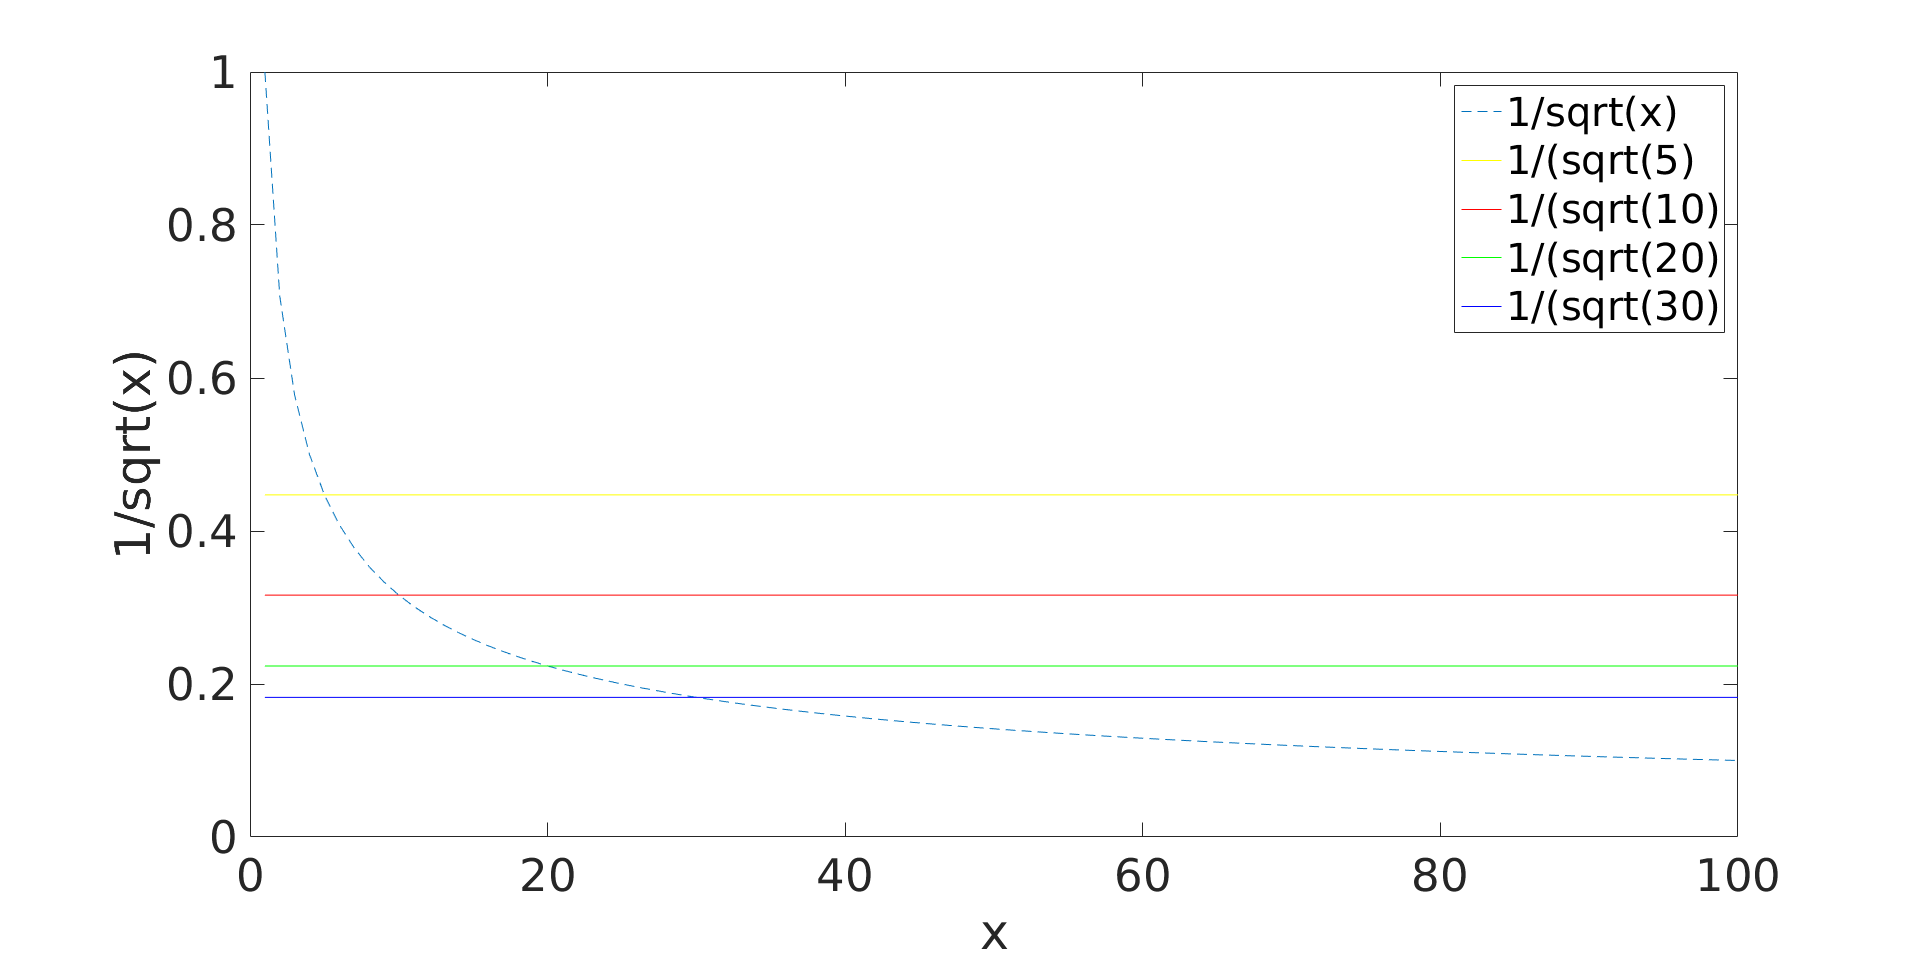
\includegraphics[width=\textwidth]{../Get_Simulation_Parameters/Number_Of_Runs.png}
				\caption{Behavior of $\frac{1}{\sqrt{x}}$}
				\label{fig:numberofruns}
			\end{figure}	
			
			In general it should hold that the more repetitions your simulation goes through, the closer its behavior gets to real world conditions. But as with many things, we want to find a good balance between \emph{correctness} and the \emph{required effort}, or a good efficiency in other words. From investigating figure \ref{fig:numberofruns} we concluded that setting $m=20$ seems like a good trade-off as at that point increasing $m>20$ further does not yield much better results anymore, relative to values of $m<20$ where performance gains are more significant.
			
			
			\item[Number of students] As the number of students is variable we simulated for a number of values, narrowing down the maximum number of students that could be supported when taking all requirements into account.
			
			
			\item[CCTV Camera] It was communicated to us that turning off the CCTV camera at the remote building location is an option. Thus we simulated every scenario once with the camera \emph{on} and once with it being \emph{off}.
		\end{description}	
		
	\section{Observation}\label{chp:observations}
		\subsection{Lecture Livestreaming Error Rate}\label{sec:errorrate}
			The most time critical application is that of the bidirectional lecture video stream. We will investigate it in this section. 
			
			The livestream demands that the packet delay remains $<100\text{ms}$. Packets that arrive later than that are dropped and contribute to the error rate. This error rate must stay below $5\%$ in order to have a functioning livestream. 
			
			Figure \ref{fig:delay} shows the average delay of the connection.
			\begin{figure}[H]
				\center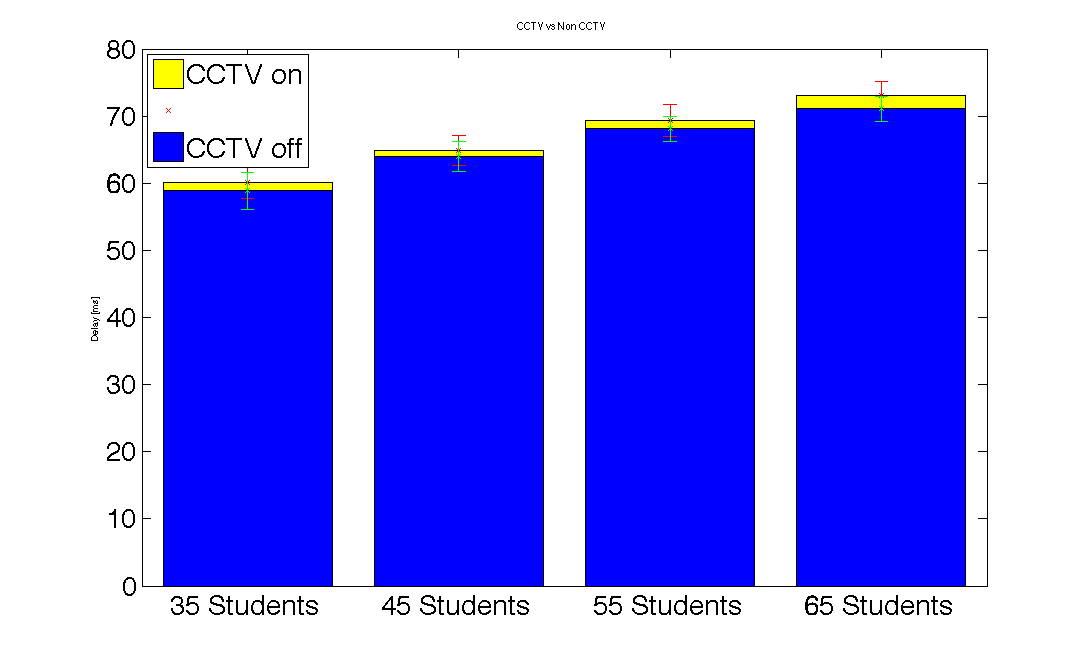
\includegraphics[width=0.8\textwidth]{../Results_Analysis/Delay/delay_combined_plot.png}
				\caption{Lecture Livestream Average Delay}
				\label{fig:delay}
			\end{figure}					
			
			We observe no surprises here. The delay increases for more users sharing the network and a turned on camera marginally increases the delay.
			
			Figure \ref{fig:errorrate} shows the behavior of the error rate. 		
			\begin{figure}[H]
				\center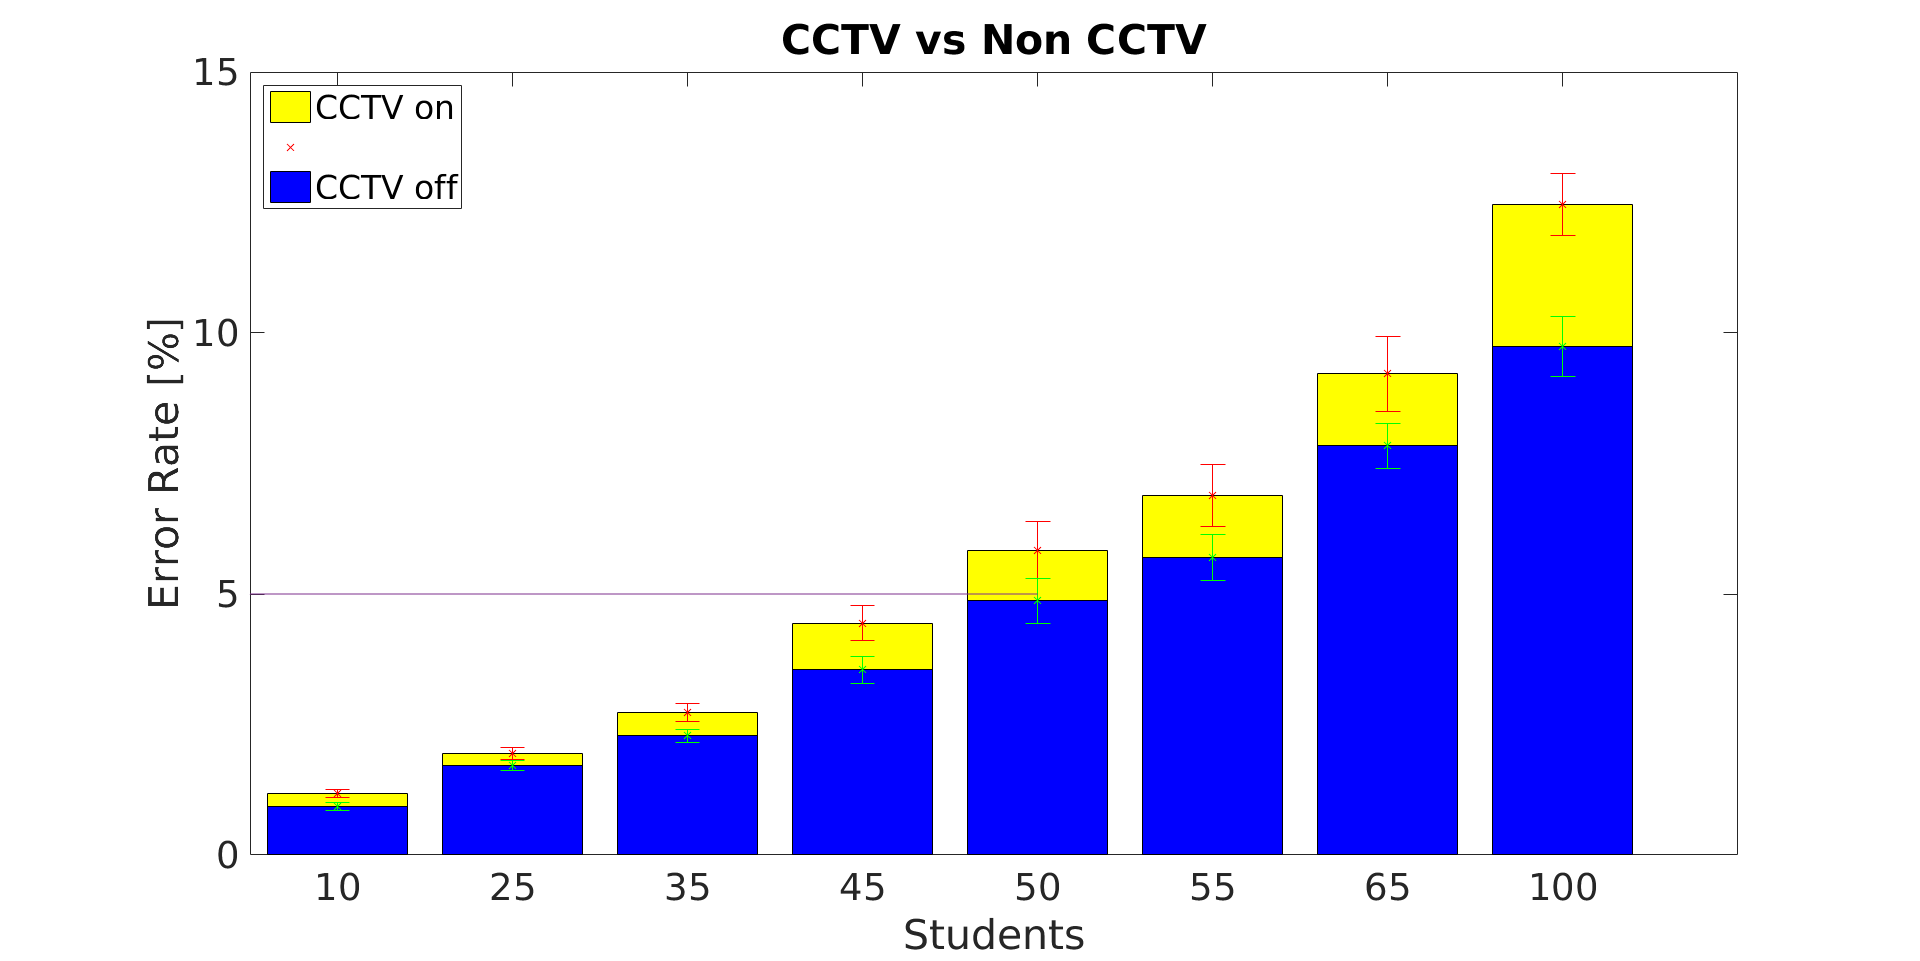
\includegraphics[width=\textwidth]{../Results_Analysis/Combining_1st_3rd_analysis/plot_all.png}
				\caption{Lecture Livestream Error Rate}
				\label{fig:errorrate}
			\end{figure}
			
			As we can see, the cut-off point seems to lie at $n=50$ students. For an online CCTV camera the error rate lies just barely outside the allowed range. For an offline camera the livestream can still go with the occasional hiccup: the confidence interval tells us that some runs' mean error rates lied beyond the $5\%$ mark and some did not.							
		
		\subsection{Web Browsing Behavior}\label{sec:http}
			The scenario's variability stems from an unknown number of students that simultaneously browses the web. Building upon results from section \ref{fig:errorrate} we decided to focus on $n~\in~\{35, 45, 55, 65\}$ students so that the range around $n=50$ where the lecture livestream starts having performance problems is depicted.
			
			\begin{figure}[H]
				\center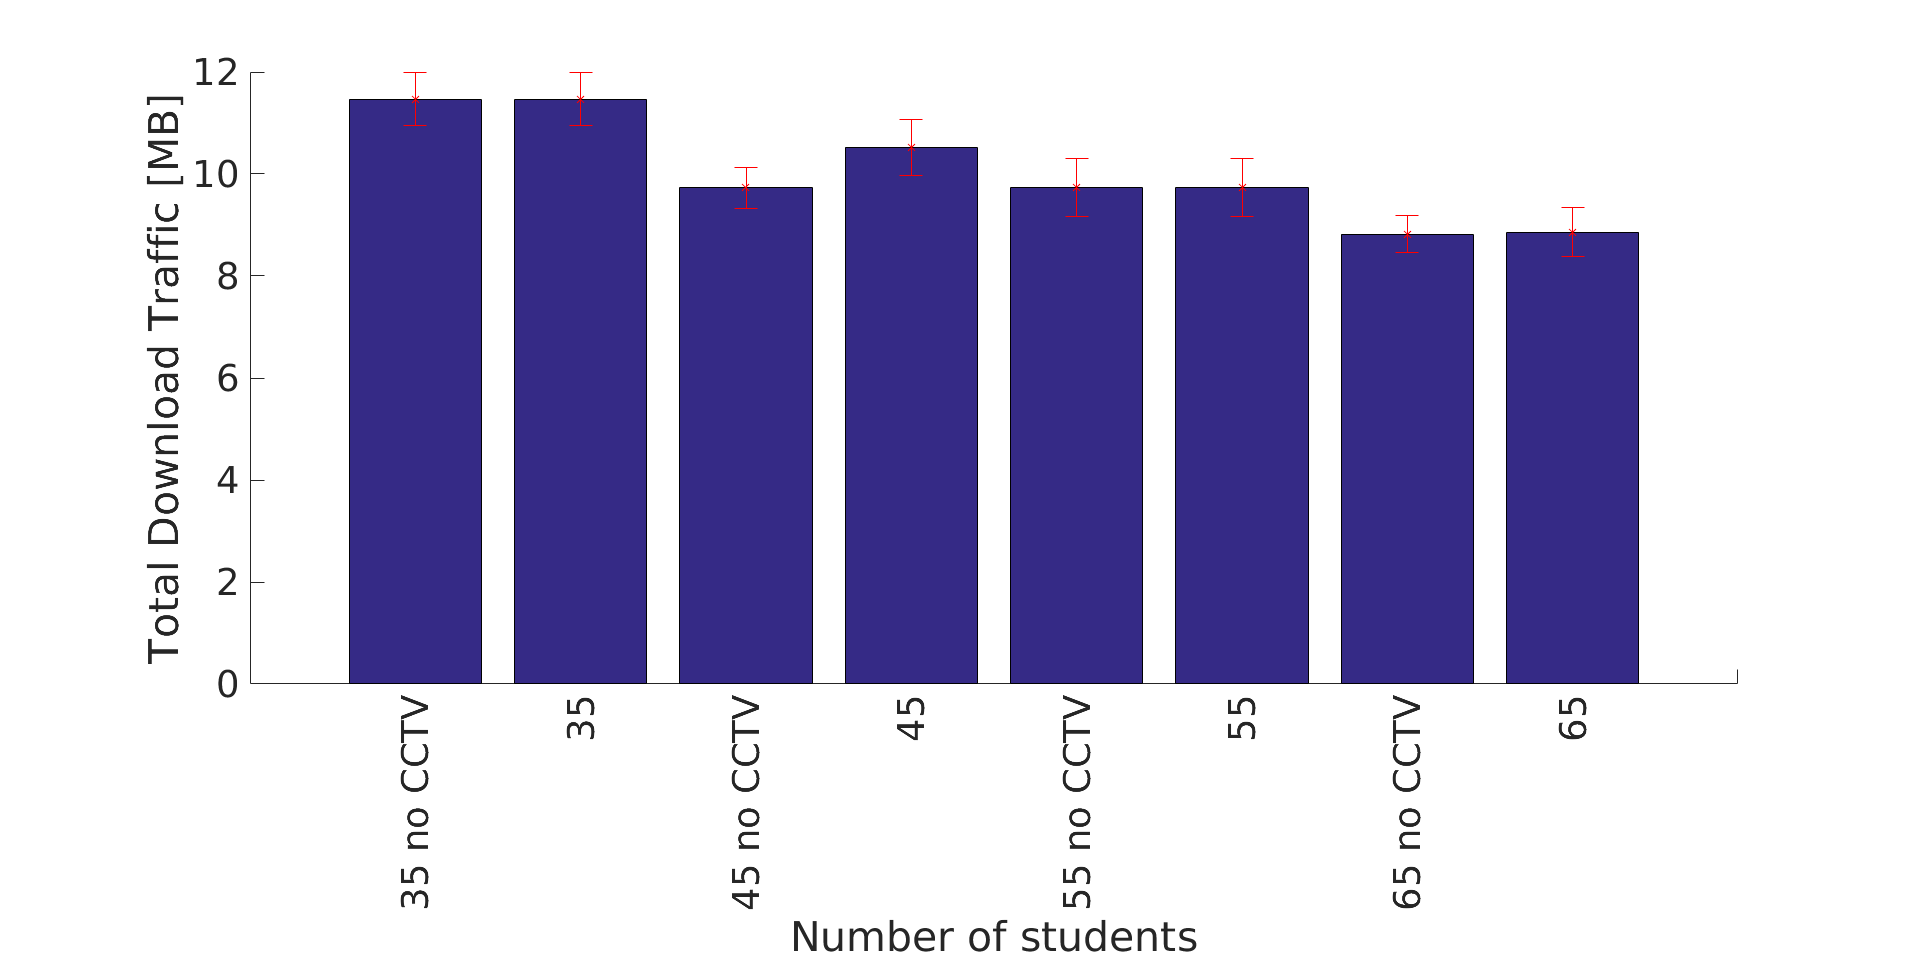
\includegraphics[width=\textwidth]{../Results_Analysis/HTTP/http.png}
				\caption{Total download traffic of an average student over $500\text{s}$}
				\label{fig:http}
			\end{figure}
			
			Figure \ref{fig:http} shows us the averaged total download traffic of any student in the eight different simulations including confidence intervals with a confidence level of $1-\alpha = 0.95$. As expected the total decreases for more users.
			
			What is interesting to observe is that turning the CCTV camera on or off does not influence the total in a significant way. For $n=45$ the total actually increases for an online camera, which seems counterintuitive at first glance. We will investigate this further in secions \ref{sec:cctvinfluence} and chapter \ref{sec:analysis}.		
			
		\subsection{File Uploading Behavior}\label{sec:ftp}		
			
		
	\chapter{Analysis}\label{sec:analysis}
		We have made many interesting observations in section \ref{chp:observations}. In this chapter we will try to analyze these observations, interpret them, evaluate the usefulness of the backup radio channel and give ideas on how to improve the scenario.				
		
		\section{Supported number of students}
		As section \ref{sec:errorrate} showed us, more than $n=50$ students can certainly not be supported, even if the camera is turned off, if we want to maintain a lecture livestream's error rate of $<5\%$. If the stream becomes noticeably erroneous, then we advise the administrator to turn off the CCTV camera. If the number of students goes far beyond $n\geq 45$, turning off the camera results in the system being able to support an additional, small number of students. Staying below this threshold, running the CCTV camera should not be a problem. Approaching $n=55$ students, given a turned off CCTV camera, the livestream will start going beyond the critical $5\%$ error rate and start having a notable packet loss.	
		
		\section{Radio link traffic}
		Many inputs to the backup radio link are known to us. Only the number of students is variable here. This section aims at breaking down what contributes to the backup radio link's traffic.
		
			\subsection{CCTV camera's influence on the generated traffic}\label{sec:cctvinfluence}
			As observed in section \ref{fig:http} the CCTV camera does not appear to affect the wireless users' throughput in a significant way. Lets recall the relevant network setup:
			
			\begin{figure}[H]
				\center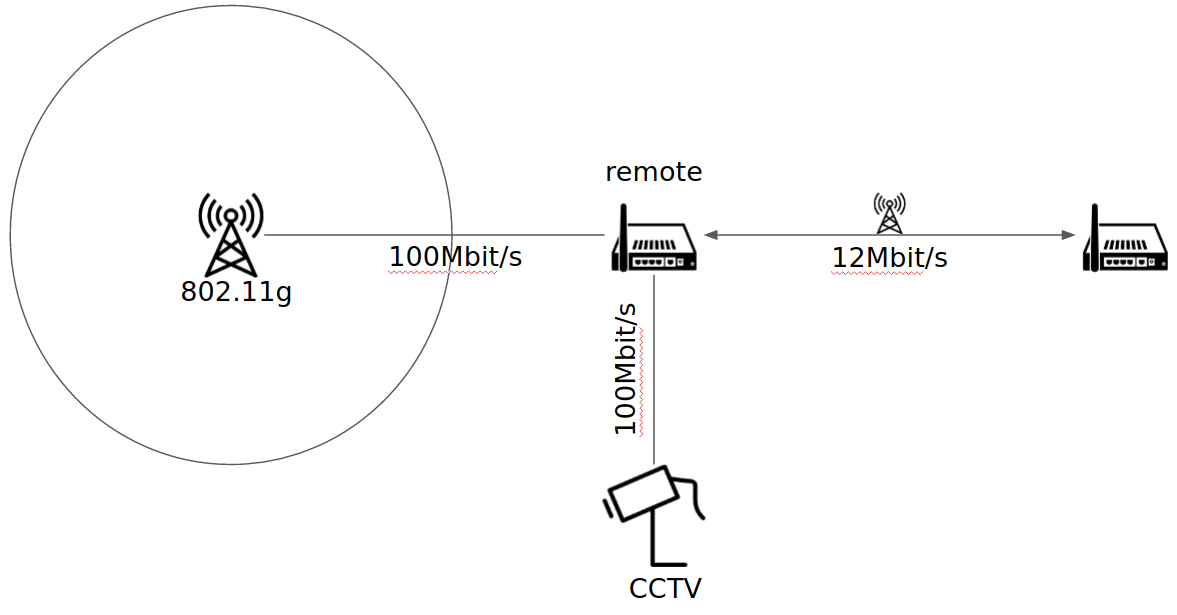
\includegraphics[width=\textwidth]{./simmodel_cctv_vs_wlan.png}
				\caption{Network model excerpt - CCTV and WLAN}
			\end{figure}
			
			Apparently CCTV and the WLAN subnetworks do not directly share a link. Their data meets at the backup radio link as both data streams travel out towards the main campus. We know the CCTV's data rate of  
			\[d_\text{\tiny CCTV}=\frac{10\text{kB}}{40\text{ms}}=\frac{2\text{MBit}}{\text{s}}\]. 
			
			We also know that the backup channel supports a bandwidth of \[B_\text{\tiny CHN}=\frac{12\text{Mbit}}{\text{s}}\]
			
			From this follows that the CCTV data stream takes up $\frac{1}{6}$ of the backup channel's bandwidth, leaving a majority of the bandwidth \[B_\text{\tiny CHN}^\text{free}=\frac{5}{6} B_\text{\tiny CHN}=\frac{1250\text{kB}}{\text{s}}\] free for the WLAN subsystem and so we can set the influence of the camera on the traffic as:
			
			\[d_\text{\tiny CCTV}=\frac{1}{6}\cdot B_\text{\tiny CHN}\]
		
			\subsection{Lecture livestream's influence on the generated traffic}
			We have knowledge about the technical details of the livestream: 
		\[d_\text{\tiny STR}^\text{1-way}=\frac{1400\text{B}}{40\text{ms}}=\frac{0.28\text{MBit}}{\text{s}}\]
		
			\[\Rightarrow d_\text{\tiny STR}=2\cdot d_\text{\tiny STR}^\text{1-way}=\frac{0.56\text{MBit}}{\text{s}}\]
			
			\[\Rightarrow d_\text{\tiny STR}=0.0467\cdot B_\text{\tiny CHN}\]
			
			\subsection{FTP upload's influence on the generated traffic}
			The constant FTP upload that takes place is more difficult to capture. FTP is an application layer protocol that operates on TCP. As such it has no knowledge of the network's current state. It passes on as much data as it wants to send, leaving the job of breaking down this data into chunks that \emph{can} actually be sent to the TCP protocol. 
			
			
			
			\subsection{Radio link throughput}
			Putting the pieces together we obtain the backup channel's average throughput:
			
			

\end{document}
